\documentclass{standalone}
\usepackage{tikz}
\usepackage{ctex,siunitx}
\usepackage{tkz-euclide}
\usepackage{amsmath}
\usetikzlibrary{patterns, calc}
\usetikzlibrary {decorations.pathmorphing, decorations.pathreplacing, decorations.shapes,}
\begin{document}
\small
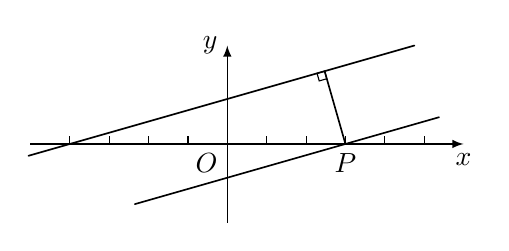
\begin{tikzpicture}[>=latex,scale=0.5]
  \draw[thin,->](-5,0)--(6,0)node[below]{$x$};
  \draw[thin,->](0,-2)--(0,2.5)node[left]{$y$};
  \tkzDefPoints{0/0/O,-0.5/1/A,3/2/B,3/0/P}
  \foreach \x in {-4,-3,-2,-1,1,2,3,4,5}
  {
    \draw[thin](\x,0)--++(0,0.2);
  }
  \tkzDefPointBy[projection=onto A--B](P)\tkzGetPoint{D}
  \tkzDefPointBy[translation=from D to A ](P)\tkzGetPoint{C}
  \tkzDrawLine[semithick,add= 1.3 and 0.5](A,B)
  \tkzDrawLine[semithick,add= 0.8 and 0.8](C,P)
  \tkzDrawSegments[semithick](P,D)
  \tkzMarkRightAngle[size=0.2](P,D,A)
  % \tkzDrawLine[semithick,add= 0.05 and 0](C,D)
  \tkzLabelPoints[below left](O)
  \tkzLabelPoints[below](P)
\end{tikzpicture}
\end{document}